\documentclass[a4paper]{book}
\usepackage{fullpage}

\usepackage[utf8]{inputenc}
\usepackage[T1]{fontenc}
\usepackage[francais]{babel}

\usepackage{latexsym}
\usepackage{fancyhdr}
\usepackage{makeidx}
\usepackage{graphics}
\usepackage{graphicx}
\usepackage{float} %
\usepackage{caption} %
\usepackage{longtable}
\usepackage{moreverb}
\usepackage{listings}

\newcommand{\altarica}{{\sc AltaRica}}

\begin{document}

\title{Master 1, Conceptions Formelles\\
Projet du module \altarica\\
Synthèse (assistée) d'un contrôleur du niveau d'une cuve}

\date{}

\author{Craeye Nathalie \and Faltrept Bérénice \and Lejeune David}

\maketitle

\chapter{Le sujet}
\section{Cahier des charges}

Le système que l'on souhaite concevoir est composé~:
\begin{itemize}
\item d'un réservoir contenant {\bf toujours} suffisamment d'eau pour alimenter l'exploitation,
\item d'une cuve,
\item de deux canalisations parfaites amont reliant le réservoir à la cuve, et permettant d'amener l'eau à la cuve,
\item d'une canalisation parfaite aval permettant de vider l'eau de la cuve,
\item chaque canalisation est équipée d'une vanne commandable, afin de réguler l'alimentation et la vidange de la cuve,
\item d'un contrôleur.
\end{itemize}

\subsection{Détails techniques}

\subsubsection{La vanne}
Les vannes sont toutes de même type, elles possèdent trois niveaux de débits correspondant à trois diamètres d'ouverture~: 0 correspond à la vanne fermée, 1 au diamètre intermédiaire et 2 à la vanne complètement ouverte. Les vannes sont commandables par les deux instructions {\tt inc} et {\tt dec} qui respectivement augmente et diminue l'ouverture. Malheureusement, la vanne est sujet à défaillance sur sollicitation, auquel cas le système de commande devient inopérant, la vanne est désormais pour toujours avec la même ouverture.

\subsubsection{La Cuve}
Elle est munie de $nbSensors$ capteurs (au moins quatre) situés à $nbSensors$ hauteurs qui permettent de délimiter $nbSensors+1$ zones. La zone 0 est comprise entre le niveau 0 et le niveau du capteur le plus bas; la zone 1 est comprise entre ce premier capteur et le second, et ainsi de suite.

Elle possède en amont un orifice pour la remplir limité à un débit de 4, et en aval un orifice pour la vider limité à un débit de 2.  

\subsubsection{Le contrôleur}
Il commande les vannes avec les objectifs suivants ordonnés par importance~:
\begin{enumerate}
\item Le système ne doit pas se bloquer, et le niveau de la cuve ne doit jamais atteindre les zones 0 ou $nbSensors$.
\item Le débit de la vanne aval doit être le plus important possible.
\end{enumerate}

On fera également l'hypothèse que les commandes ne prennent pas de temps, et qu'entre deux pannes et/ou cycle {\em temporel}, le contrôleur à toujours le temps de donner au moins un ordre. Réciproquement, on fera l'hypothèse que le système à toujours le temps de réagir entre deux commandes.

\subsubsection{Les débits}
Les règles suivantes résument l'évolution du niveau de l'eau dans la cuve~:
\begin{itemize}
\item Si $(amont > aval)$ alors au temps suivant, le niveau aura augmenté d'une unité.
\item Si $(amont < aval)$ alors au temps suivant, le niveau aura baissé d'une unité.
\item Si $(amont = aval = 0)$ alors au temps suivant, le niveau n'aura pas changé.
\item Si $(amont = aval > 0)$ alors au temps suivant, le niveau pourra~:
  \begin{itemize}
  \item avoir augmenté d'une unité,
  \item avoir baissé d'une unité,
  \item être resté le même.
  \end{itemize}
\end{itemize}

\section{L'étude}

\subsection{Rappel méthodologique}
Comme indiqué en cours, le calcul par point fixe du contrôleur est exact, mais l'opération de projection effectuée ensuite peut perdre de l'information et générer un contrôleur qui n'est pas satisfaisant. Plus précisemment, le contrôleur \altarica\ généré~:
\begin{itemize}
\item ne garanti pas la non accessibilité des \emph{Situations Redoutées}.
\item ne garanti pas l'absence de \emph{nouvelles situations de blocages}.
\end{itemize}

Dans le cas ou il existe toujours \emph{des situations de blocages ou redoutées}, vous pouvez au choix~:
\begin{enumerate}
\item Corriger manuellement le contrôleur calculé (sans doute très difficile).
\item Itérer le processus du calcul du contrôleur jusqu'à stabilisation du résultat obtenu. 
  \begin{itemize}
  \item Si le contrôleur obtenu est sans blocage et sans situation redoutée, il est alors correct.
  \item Si le contrôleur obtenu contient toujours des blocages ou des situations redoutées, c'est que le contrôleur initial n'est pas assez performant, mais rien de garanti que l'on soit capable de fournir ce premier contrôleur suffisemment performant.
  \end{itemize}
\end{enumerate}

{\bf Remarque} : Pour vos calculs, vous pouvez utiliser au choix les commandes~:
\begin{itemize}
\item {\tt altarica-studio xxx.alt xxx.spe}
\item {\tt arc -b xxx.alt xxx.spe}
\item {\tt make} pour utiliser le fichier GNUmakefile fourni.
\end{itemize}

\subsection{Le travail a réaliser}

Avant de calculer les contrôleurs, vous devez répondre aux questions suivantes.
\begin{enumerate}
\item Expliquez le rôle de la constante $nbFailures$ et de la contrainte, présente dans le composant {\tt System}, $nbFailures >= (V[0].fail + V[1].fail + V[2].fail)$.
\item Expliquez le rôle du composant {\tt ValveVirtual} et de son utilisation dans le composant {\tt CtrlVV}, afin de remplacer le composant {\tt Ctrl} utilisé en travaux dirigés.
\end{enumerate}

L'étude consiste à étudier le système suivant deux paramètres~:
\begin{enumerate}
\item $nbFailures$~: une constante qui est une borne pour le nombre de vannes pouvant tomber en panne.
\item Le contrôleur initial qui peut être soit {\tt Ctrl}, soit {\tt CtrlVV}.
\end{enumerate}

Pour chacun des huit systèmes étudiés, vous devez décrire votre méthodologie pour calculer les différents contrôleurs et répondre aux questions suivantes~:

\begin{enumerate}
\item Est-il possible de contrôler en évitant les blocages et les situations critiques ?
\item Si oui, donnez quelques caractéristiques de ce contrôleur, si non, expliquez pourquoi.
\item Est-il possible de contrôler en optimisant le débit aval et en évitant les blocages et les situations critiques ?
\item Si oui, donnez quelques caractéristiques de ce contrôleur, si non, expliquez pourquoi.
\end{enumerate}


\chapter{Le rapport}

Pour les deux questions concernant l'étude des constante et composants, nous avons analysé essentiellement le fichier GNUmakefile à la racine du projet, mais aussi les fichiers System.alt, Parameters.alt, tank.alt, test.alt, et CtrlVV.alt.
En effet nous avons remarqué, dans le fichier GNUmakefile, qu'à l'utilisation de la commande "make" on génère toutes les configurations possibles du système sur lequel nous travaillons : 
une première boucle for assure la génération des fichiers pour tous les contrôleurs (Ctrl et CtrlVV) ; puis une deuxième boucle for va produire, pour chacun d'entre eux, les différents systèmes associés aux différents nombres de pannes possibles (i.e : 0, 1, 2 et 3). \\

Pour les questions portant sur l'analyse des 8 systèmes, nous avons utilisé les outils suivants, et dans cet ordre : GNUmakefile (via la commande $make$) puis Altarica-Studio (via la commande $altarica-studio Alt/System.alt Spec/System.spe$) à la racine du projet. De plus, pour obtenir l'affichage, dans les fichiers résultats générés, du nombre de deadlock traçables dans certains systèmes à partir de certaines itérations, nous avons modifié la commande show dans $System.spe$ en lui rajoutant en argument la propriété tr\_deadlock :  {\tt show(any\_s, any\_t, deadlock, tr\_deadlock, NC, SR , out0, out1, out2, CtrlCanControl,CCoupGagnant, CCoupGagnantUtile) > 'Res/\$NODENAME.res';}. Pour finir, pour pouvoir analyser les traces des deadlock dans l'onglet {\tt Graph}, via la commande $dot(any\_s, tr\_deadlock)$, sous Altarica-Studio, nous modifions les variables $PANNES$, $ITERATIONS$ et $CONTROLEURS\_INIT$ dans le GNUmakefile à la racine du projet de sorte que nous retrouvions plus vite la configuration du système avec deadlocks que l'on souhaitait étudiée.

\section{Rôle de la constante {\tt nbFailures} (2 points)}

$nbFailures$ est la constante qui récupère le nombre de pannes prédéfini au lancement d'une configuration du système. En effet, elle est initialisée en prenant la valeur de la variable $nbPannes$ (cf GNUmakefile) dans le système en cours. \\
La contrainte, et assertion, du composant {\tt System} $nbFailures >= (V[0].fail + V[1].fail + V[2].fail)$ permet d'assurer que le modèle lancé par l'utilisateur a une configuration cohérente. En effet, elle vérifie que le nombre de valves en panne dans le modèle en cours sera compris entre 0 (meilleur cas : il n'y aurait aucune valve en panne) et 3 (pire cas : les trois valves existantes du système sont en panne). \\


\section{Rôle des composants {\tt ValveVirtual} et {\tt CtrlVV} (4 points)}

$ValveVirtual$ est le composant permettant de simuler une valve parfaite, autrement dit une valve qui ne peut pas tomber en panne. Le composant {\tt ValveVirtual} étant intégré au modèle, via {\tt CtrlVV}, on peut alors confirmer la cohérence du modèle indépendemment de la gestion des pannes. \\
$CtrlVV$ est le composant qui, en remplaçant le contrôleur {\tt Ctrl}, contrôle le système. Ce qui le distingue du précédent est sa capacité à gérer en parallèle du système, une simulation du système dans laquelle aucune panne n'est possible. \\
Lorsque {\tt CtrlVV} agit sur une des valves du système réel, il reproduit la même action sur la valve correspondante du simulateur. \\
Si les conséquences dans la cuve réelle sont différentes de celles dans la cuve simulée, alors il détecte que la valve concernée est défaillante.


\section{Résultats avec le contrôleur initial {\tt Ctrl}}

\subsection{Calcul d'un contrôleur}

\subsubsection{Avec 0 défaillance (1 point)}
\lstinputlisting{Res/System0FCtrl.res}
\lstinputlisting{Res/System0FCtrl0F1I.res}
\lstinputlisting{Res/System0FCtrl0F2I.res}
\lstinputlisting{Res/System0FCtrl0F3I.res}
\lstinputlisting{Res/System0FCtrl0F4I.res}
\paragraph{Interprétation des résultats}

On observe que, excepté la première, les différentes itérations sont toutes identiques. De plus, dans cette configuration, nous notons que le système n'a aucun deadlock et que les situations redoutées n'existent plus après la première tentative. Nous en concluons que le raffinement après l'itération 1 est concluant et permet d'obtenir un système que l'on peut supposer fiable.

\begin{itemize}
	\item Oui. À partir de l'itération 1, il n'y a ni situation critique et ni état puit. Dans cette situation, CtrlCanControl parvient à contrôler 27 transitions.
	\item Out2 étant la sortie utilisée dans le plus de situations (ou sommets) et ayant un nombre de situations critiques nul, le modèle est déjà optimal.
\end{itemize}

\subsubsection{Avec 1 défaillance (1 point)}
\lstinputlisting{Res/System1FCtrl.res}
\lstinputlisting{Res/System1FCtrl1F1I.res}
\lstinputlisting{Res/System1FCtrl1F2I.res}
\lstinputlisting{Res/System1FCtrl1F3I.res}
\lstinputlisting{Res/System1FCtrl1F4I.res}
\paragraph{Interprétation des résultats}

Nous voyons que comparée à la version 0 défaillance, la configuration initiale a beaucoup plus de situations redoutées possibles, ce qui nous paraît normal étant donné que le modèle a une valve défaillante et donc de nouvelles situations à gérer. \\
À la première itération, nous remarquons que des états puits sont reconnus, et que les sommets pour lesquels le niveau d'eau est critique sont tous des deadlocks puisque SR est équivalent à deadlock. \\ 
Or, en utilisant Altarica-Studio, on s'aperçoit que la trace des deadlock ne nous mènent qu'à 4 sommets. En affichant le graphe avec la commande $dot(any\_s, tr\_deadlock)$, on découvre que ces 4 cas recouvrent les situations où le niveau de l'eau dans la cuve est débordant.

\begin{figure}[H]
  \centering
  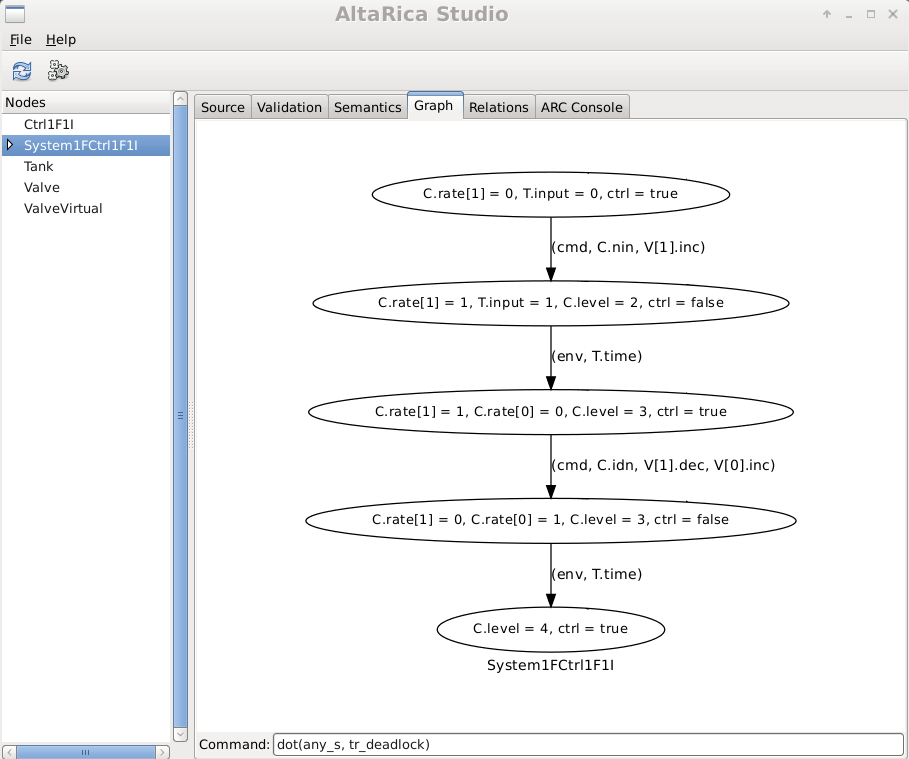
\includegraphics[width=14cm]{img/CtrlF1I1.png}
  \caption{tr\_deadlock dans le contrôleur CtrlF1I1}
\end{figure}

\begin{itemize}
	\item En ayant une valve défaillante, on peut contrôler toutes les situations exceptées les débordements de cuves qui peuvent arriver quelle que soit la valve abîmée. Dans ce cas, on doit trouver une solution spécifique à ce problème : par exemple, garder une ouverture en haut de la cuve qui entrainerait une perte de l'eau le temps que l'on répare la valve. Donc non.
	\item Comme nous le voyons sur l'image ci-dessus : à aucun moment le débit aval n'intervient sur les trajets partant du sommet initial et arrivant à une situation bloquée (deadlock). Donc non.
\end{itemize}

\subsubsection{Avec 2 défaillances (1 point)}
\lstinputlisting{Res/System2FCtrl.res}
\lstinputlisting{Res/System2FCtrl2F1I.res}
\lstinputlisting{Res/System2FCtrl2F2I.res}
\lstinputlisting{Res/System2FCtrl2F3I.res}
\lstinputlisting{Res/System2FCtrl2F4I.res}
\paragraph{Interprétation des résultats}

Nous remarquons qu'à l'initialisation, il n'y a pas de deadlock. Par contre, le nombre de situations redoutées accessibles est grand. \\
À chaque itération, on obtient 2 deadlock traçables. Via Altarica-Studio, nous avons constaté que le problème survient lorsque le niveau de l'eau dans la cuve vaut 2 et que les 2 valves cassées le font augmenter.

\begin{figure}[H]
  \centering
  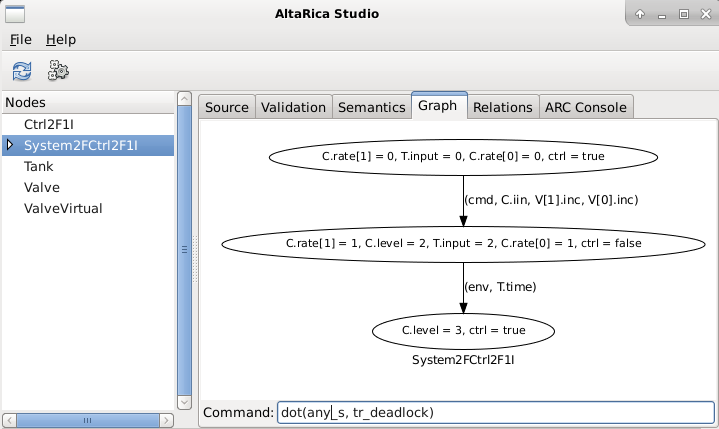
\includegraphics[width=14cm]{img/CtrlF2I1.png}
  \caption{tr\_deadlock dans le contrôleur CtrlF2I1}
\end{figure}

\begin{itemize}
	\item Non car d'après les résultats, il y a toujours les 2 mêmes deadlock traçables et un nombre d'états puits se stabilisant autour de 270.
	\item 
\end{itemize}

\subsubsection{Avec 3 défaillances (1 point)}
\lstinputlisting{Res/System3FCtrl.res}
\lstinputlisting{Res/System3FCtrl3F1I.res}
\lstinputlisting{Res/System3FCtrl3F2I.res}
\lstinputlisting{Res/System3FCtrl3F3I.res}
\lstinputlisting{Res/System3FCtrl3F4I.res}
\paragraph{Interprétation des résultats}

En rapport avec le très grand nombre de situations à traiter, le nombre de coups contrôlables et gagnants n'est pas très important dans la configuration initiale mais nous pouvons noter que ce ratio s'améliore après la première itération.

\begin{itemize}
	\item Oui car le système semble gérer un peu les défaillances vu que les deadlocks diminuent jusqu'à 27 et qu'à chaque itération il y en a 2 qui sont traçables.
	\item 
\end{itemize}

\subsection{Calcul des contrôleurs optimisés (2 points)}

\section{Résultats avec le contrôleur initial {\tt CtrlVV}}

\subsection{Calcul d'un contrôleur}

\subsubsection{Avec 0 défaillance (1 point)}
\lstinputlisting{Res/System0FCtrlVV.res}
\lstinputlisting{Res/System0FCtrlVV0F1I.res}
\lstinputlisting{Res/System0FCtrlVV0F2I.res}
\lstinputlisting{Res/System0FCtrlVV0F3I.res}
\lstinputlisting{Res/System0FCtrlVV0F4I.res}
\paragraph{Interprétation des résultats}

Comme attendu, lors des itérations, nous n'avons aucune situation redoutée puisque nous traitons un cas sans défaillance. \\ 
On peut donc supposer que l'on est sur un système parfait pour ce nombre de défaillance. Nous remarquons aussi que nous avons les mêmes valeurs que lors de l'utilisation du contrôleur classique avec aucune défaillance possible, seul le nombre de transitions varie.

\begin{itemize}
	\item Oui, effectivement nous voyons que nous sommes sans situation redoutée mais que CtrlCanControl n'est que de 8.
	\item Ce cas étant similaire à la première configuration étudiée, nous en tirons la conclusion que le modèle est déjà optimal.
\end{itemize}

\subsubsection{Avec 1 défaillance (1 point)}
\lstinputlisting{Res/System1FCtrlVV.res}
\lstinputlisting{Res/System1FCtrlVV1F1I.res}
\lstinputlisting{Res/System1FCtrlVV1F2I.res}
\lstinputlisting{Res/System1FCtrlVV1F3I.res}
\lstinputlisting{Res/System1FCtrlVV1F4I.res}
\paragraph{Interprétation des résultats}

Dans la nouvelle configuration initiale, le nombre de situations, {\tt any\_s}, valant 1201, nous pouvons voir que ce nombre est 6 fois plus grand que l'ensemble des états au départ du même système sans défaillance.
Dans ce système, c'est seulement à la suite de 3 itérations que le système est totalement fiable (sans aucune situation redoutée), probablement parce que c'est le temps qu'il met à corriger les trois défaillances possibles (car 1 seule défaillance dans le système).

\begin{itemize}
	\item Oui, nous pouvons optimiser en évitant les situations redoutée : c'est exactement le rôle de {\tt CtrlVV}. L'action sur la valve défaillante réelle sera rectifiée par ce dernier. C'est pourquoi qu'au fur-et-à mesure des itérations le nombre de deadlock d'abord augmente puis tend à disparaître.
	\item 
\end{itemize}

\subsubsection{Avec 2 défaillances (1 point)}
\lstinputlisting{Res/System2FCtrlVV.res}
\lstinputlisting{Res/System2FCtrlVV2F1I.res}
\lstinputlisting{Res/System2FCtrlVV2F2I.res}
\lstinputlisting{Res/System2FCtrlVV2F3I.res}
\lstinputlisting{Res/System2FCtrlVV2F4I.res}
\paragraph{Interprétation des résultats}

Encore une fois, le nombre de situations à traiter double par rapport au système initial précédent. Après la première itération le modèle s'est assez raffiné pour qu'il n'y ait plus aucune situations redoutées.

\begin{itemize}
	\item Oui, c'est le rôle des premières itérations. C'est d'ailleurs pourquoi au fur-et-à mesure des itérations le nombre de deadlock d'abord augmente puis tend à disparaître. Nous pouvons également dire que dès la troisième itéraion, le système n'a plus qu'une situation atteignable, et elle est gagnante.
	\item Non car d'après les résultats, dans les situations fiables de ce systèmes le débit aval n'est pas optimal car c'est $out0$ qui vaut $any\_s$.
\end{itemize}

\subsubsection{Avec 3 défaillances (1 point)}
\lstinputlisting{Res/System3FCtrlVV.res}
\lstinputlisting{Res/System3FCtrlVV3F1I.res}
\lstinputlisting{Res/System3FCtrlVV3F2I.res}
\lstinputlisting{Res/System3FCtrlVV3F3I.res}
\lstinputlisting{Res/System3FCtrlVV3F4I.res}
\paragraph{Interprétation des résultats}

La configuration initiale, reconnait bien les 27 coups possibles du systèmes car il y a 27 $CtrlCanControl$. Comme il y a beaucoup plus de situations possibles alors il y a également beaucoup de $NC$.

\begin{itemize}
	\item Oui, c'est le rôle de la première itération. Dès la deuxième itération, le nombre de situations redoutées est à 0 et il n'y a plus qu'une situation gagnante qui est atteignable.
	\item Non car d'après les résultats, dans les situations fiables de ce systèmes le débit aval n'est pas optimal car c'est $out0$ qui vaut $any\_s$.
\end{itemize}

\subsection{Calcul des contrôleurs optimisés (2 points)}

\section{Conclusion (2 points)}

Finalement, nous ne sommes pas parvenus à aboutir à ce projet. Durant l'analyse des différents systèmes, nous nous sommes plusieurs fois demandés quelles étaient la définition d'une itération et la signification de l'optimisation du débit aval sans parvenir à des définitions/conclusions précises. Nous avons donc malheureusement travaillé sur plusieurs suppositions.\\
De plus, nous n'avons pas compris si nous devions modifier manuellement les contrôleurs générés dans le dossier $Controleurs$ lorsqu'ils avaient des deadlocks et si oui de quelle manière (sachant que lors des TD sur le système {\tt Building} nous avions vu qu'en rajoutant la trace de propriétés de sûreté au système, on devait rajouter des contraintes dans le modèle via variables et/ou synchronisation d'évènements).\\
En nous basant sur nos connaissances d'Altarica-Studio, nous avons pu exposer des éléments de réponses malgré une exploitation incomplète de ces résultats. \\
En revanche, notre attention s'étant focalisée sur le fonctionnement du projet, nous avons ainsi assimilé le rôle des composants dans le système, et plus généralement, la signification des opérateurs et l'importance de la robustesse à apporter dans un modèle. \\

\end{document}
